\documentclass{article}
\usepackage{tikz}
\usepackage{caption}
\begin{document}

\begin{figure}[h!]
\centering

% (a) Chaîne alimentaire
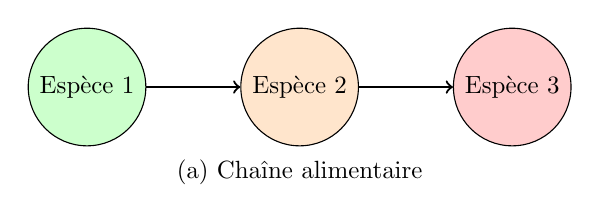
\begin{tikzpicture}[scale=0.9, every node/.style={scale=0.9}]
\node[draw, circle, fill=green!20] (A) at (0,0) {Espèce 1};
\node[draw, circle, fill=orange!20] (B) at (3,0) {Espèce 2};
\node[draw, circle, fill=red!20] (C) at (6,0) {Espèce 3};
\draw[->, thick] (A) -- (B) node[midway, above] {};
\draw[->, thick] (B) -- (C) node[midway, above] {};
\node at (3,-1.2) {(a) Chaîne alimentaire};
\end{tikzpicture}

\vspace{1cm}

% (b) Deux prédateurs - une proie
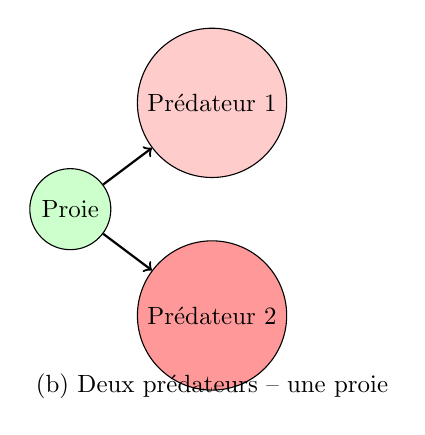
\begin{tikzpicture}[scale=0.9, every node/.style={scale=0.9}]
\node[draw, circle, fill=green!20] (A) at (0,0) {Proie};
\node[draw, circle, fill=red!20] (B) at (2,1.5) {Prédateur 1};
\node[draw, circle, fill=red!40] (C) at (2,-1.5) {Prédateur 2};
\draw[->, thick] (A) -- (B);
\draw[->, thick] (A) -- (C);
\node at (2,-2.5) {(b) Deux prédateurs -- une proie};
\end{tikzpicture}

\vspace{1cm}

% (c) Un prédateur - deux proies
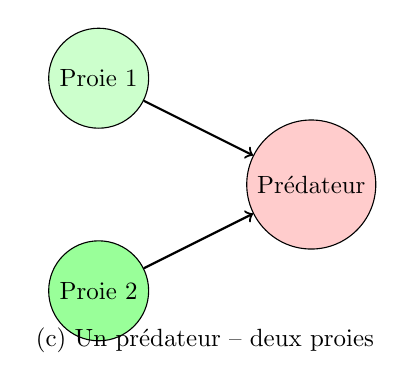
\begin{tikzpicture}[scale=0.9, every node/.style={scale=0.9}]
\node[draw, circle, fill=green!20] (A) at (0,1.5) {Proie 1};
\node[draw, circle, fill=green!40] (B) at (0,-1.5) {Proie 2};
\node[draw, circle, fill=red!20] (C) at (3,0) {Prédateur};
\draw[->, thick] (A) -- (C);
\draw[->, thick] (B) -- (C);
\node at (1.5,-2.2) {(c) Un prédateur -- deux proies};
\end{tikzpicture}

\vspace{1cm}

% (d) Chaîne alimentaire avec omnivorie
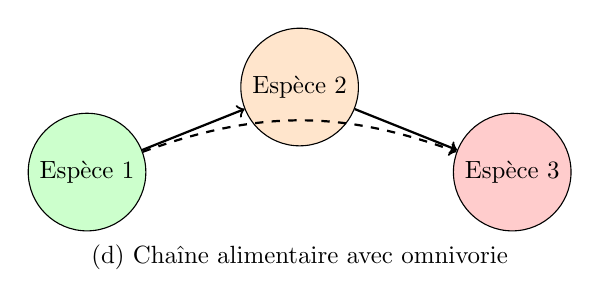
\begin{tikzpicture}[scale=0.9, every node/.style={scale=0.9}]
\node[draw, circle, fill=green!20] (A) at (0,0) {Espèce 1};
\node[draw, circle, fill=orange!20] (B) at (3,1.2) {Espèce 2};
\node[draw, circle, fill=red!20] (C) at (6,0) {Espèce 3};
\draw[->, thick] (A) -- (B);
\draw[->, thick] (B) -- (C);
\draw[->, thick, dashed] (A) to[bend left=20] (C); % Omnivorie
\node at (3,-1.2) {(d) Chaîne alimentaire avec omnivorie};
\end{tikzpicture}

\vspace{1cm}

% (e) Boucle (cycle)
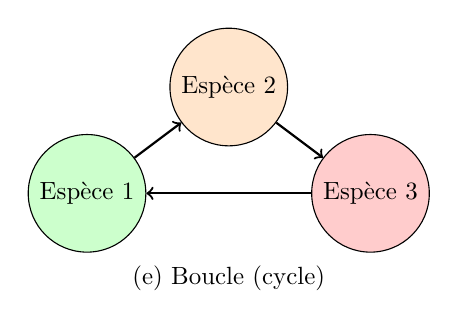
\begin{tikzpicture}[scale=0.9, every node/.style={scale=0.9}]
\node[draw, circle, fill=green!20] (A) at (0,0) {Espèce 1};
\node[draw, circle, fill=orange!20] (B) at (2,1.5) {Espèce 2};
\node[draw, circle, fill=red!20] (C) at (4,0) {Espèce 3};
\draw[->, thick] (A) -- (B);
\draw[->, thick] (B) -- (C);
\draw[->, thick] (C) -- (A);
\node at (2,-1.2) {(e) Boucle (cycle)};
\end{tikzpicture}

\caption{Schémas des différents types d’interactions proie-prédateur entre trois espèces. Les flèches indiquent « est mangé par » ou « interaction de prédation ».}
\end{figure}

\end{document}
